\documentclass[border=10pt]{standalone}
\usepackage{tikz}
\begin{document}
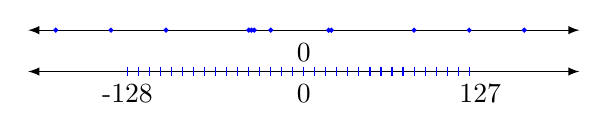
\begin{tikzpicture}[scale=0.35]
  % Data points (continuous values)
  \begin{scope}[yshift=1.5cm]
    \draw[latex-latex] (-10,0) -- (10,0);
    \foreach \x in {-9, -7, -5, -2, -1.9, -1.8, -1.2, 0.9, 1, 4, 6, 8}
      \draw[blue, fill=blue] (\x,0) circle (2pt);
    \node at (0,-0.8) {0};
  \end{scope}
  % INT8 number line (evenly spaced ticks)
  \draw[latex-latex] (-10,0) -- (10,0);
  \foreach \x in {-128,-120,...,127}
    \draw[shift={(\x/20,0)},color=blue] (0pt,5pt) -- (0pt,-5pt);
  \node at (-6.4,-0.8) {-128};
  \node at (0,-0.8) {0};
  \node at (6.4,-0.8) {127};
\end{tikzpicture}
\end{document}
